\chapter{Implementation and Build}

\section{Designing and Prototyping}
We designed the prototype of the circuit on breadboards which included the microcontroller, radio module and an oled display.

\begin{itemize}
	\item We used an atmega328p microcontroller as the library we needed for creating the mesh network with NRF24L01+ radio module was easily available for it.
	
	\item We added an oled display for testing and debugging purposes and is not intended to be a part of our final product.

	\item The breadboard circuit also had a 1117 3.3v regulator to supply the NRF radio module and the oled display.
	
	\item Programming the ATmega $\mu$C was done using FTDI USB to serial converter. The ATmega has an Arduino pro mini 8Mhz bootloader on it.
	
	\item We have used an 8Mhz crystal since we planed to reduce the supply voltage and lower clock speeds are required to reduce the supply voltage to the $\mu$C.
	
\end{itemize}	

\vspace{20pt}

\includegraphics[scale=0.05]{Breadboard.jpg}
\includegraphics[scale=0.05]{Breadboard2.jpg}

\pagebreak

\subsection{Radio Module Selection}

\begin{itemize}
	\item \textbf{ZigBee, Lora and the NRF24L01} were the suitable choice of wireless communication modules/protocols for our project. 
	\item \textbf{ZigBee} offered a easy to use mesh network setup, low power consumption and robust communication protocol. But ZigBee was cost prohibitive for creating many inexpensive devices. 
	\item \textbf{Lora} offered long range but had a nascent ecosystem and it too was cost prohibitive for creating many inexpensive devices.
	\item \textbf{NRF24L01+} modules offered a decent range had a resonable networking ecosystem developed for it and was very cost effective for creating low cost modules.
\end{itemize}	

\subsection{Low Power Considerations}
As we were making a battery powered device the current consumed should be as low as possible to maximize the battery life.
We desired a battery life of 3-12 months before the battery needs to be replaced. Hence to reduce the active and standby current of our circuit we took the following steps.

\begin{itemize}	
\item When the device is not transmitting the microcontroller and the radio module go into a deep sleep state. The current consumption reduces to \textbf{80$\mu$A}. 
\begin{itemize}
	\item \textbf{50$\mu$A} is used by the PIR sensor when motion is not detected. (150$\mu$A when motion is detected)
	\item \textbf{20$\mu$A} is the quiescent current of the voltage regulator
	\item \textbf{9$\mu$A} is the current consumption of the ATmega $\mu$C
	\item \textbf{1$\mu$A} is taken by the nrf module in the \textbf{deep sleep} state
\end{itemize}

\item We have taken various measures to reduce the power consumption of the ATmega $\mu$C.
	\begin{enumerate}
		\item Put the processor to power down mode. This is the most power efficient sleep mode. This disconnects the clock from the CPU, flash memory, IO ports, ADC. It also disconnects the external crystal oscillator and the timer oscillator. BOD is also disabled. The only way to wake up the $\mu$C is by WDT or by external interrupts.
		\item Arrange to wake the processor from sleep only when needed based on watchdog timer overflow and interrupt by the PIR sensor
		\item Run the processor at a lower frequency (8Mhz)
		\item Run the processor at a lower voltage (3V) (This will also reduce the number of batteries to be used as the supply voltage reduces)
		\item Turn off unneeded internal modules in software (eg. SPI, I2C, Serial, ADC). This will reduce the power consumption $\mu$C is awake. They are disabled by default in the sleep state
		\item Turn off brownout detection
		\item Turn off the Analog-to-Digital converter (ADC). This will reduce the power consumption $\mu$C is awake. It is disabled by default in the sleep state
		\item Set not required pins to output
	\end{enumerate} 

\item We needed a voltage regulator to reduce and regulate the supply voltage from the battery. Standard voltage regulators like the LM117 consume about 5mA operating current. Moreover the dropout voltage is too high which reduces the efficiency and also increases the voltage needed to be supplied to the device hence increasing the number of batteries.
We decided to use \textbf{TC1014-3.0V} which is a low dropout voltage, low quiecent current voltage regulator. This enabled our quiescent current of the regulator to be as low as \textbf{17$\mu$A} and it reduced the dropout voltage to \textbf{200mV}.
We purchaced the voltage regulators online from \url{tanotis.com}.

When motion is detected the device wakes up from its deep sleep state using interrupts and then transmits the required information and goes back to its deep sleep state. During this state the current consumption increases to \textbf{18mA} for about 2 seconds before the device goes back to sleep. out of these 18mA, 14.5mA is used by the NRF module and 3.5mA by the microcontroller.
\end{itemize}

\section{PCB Design}
The board has the following features
\begin{itemize}
	\item Programming interface for both serial (Arduino) as well as ISP programming
	\item Headers for RTC, NRF radio module and Oled display
	\item Onboard LDO and ultra low quiescent current voltage regulator for battery supply (TC1014-3.0V)
\end{itemize}

We used the smallest footprint components which was practical to hand assemble so that we could make the device smaller. All the resistors and capacitors are of \textbf{0805} package, ATmega is \textbf{TQFP} package, the voltage regulator is \textbf{SOT-5} package.
\\
We needed to make multiple such boards and they needed to be double sided to support the high package density. Also the lead width is small for TQFP and SOT packages. The lead width is 0.3mm-0.45mm for TQFP.
The lead pitch is 0.8mm for TQFP. 
\\Hence for these reasons we decided to get the PCBs professionally manufactured from a PCB prototyping service (\url{PCBway.com}).

\begin{center}
		\includegraphics[scale=0.31]{EaglePCB.png}		
		\hspace{10pt}
		\includegraphics[scale=0.075]{PCB_1.jpg}
		
		Eagle CAD Design and Manufactured PCB
		
		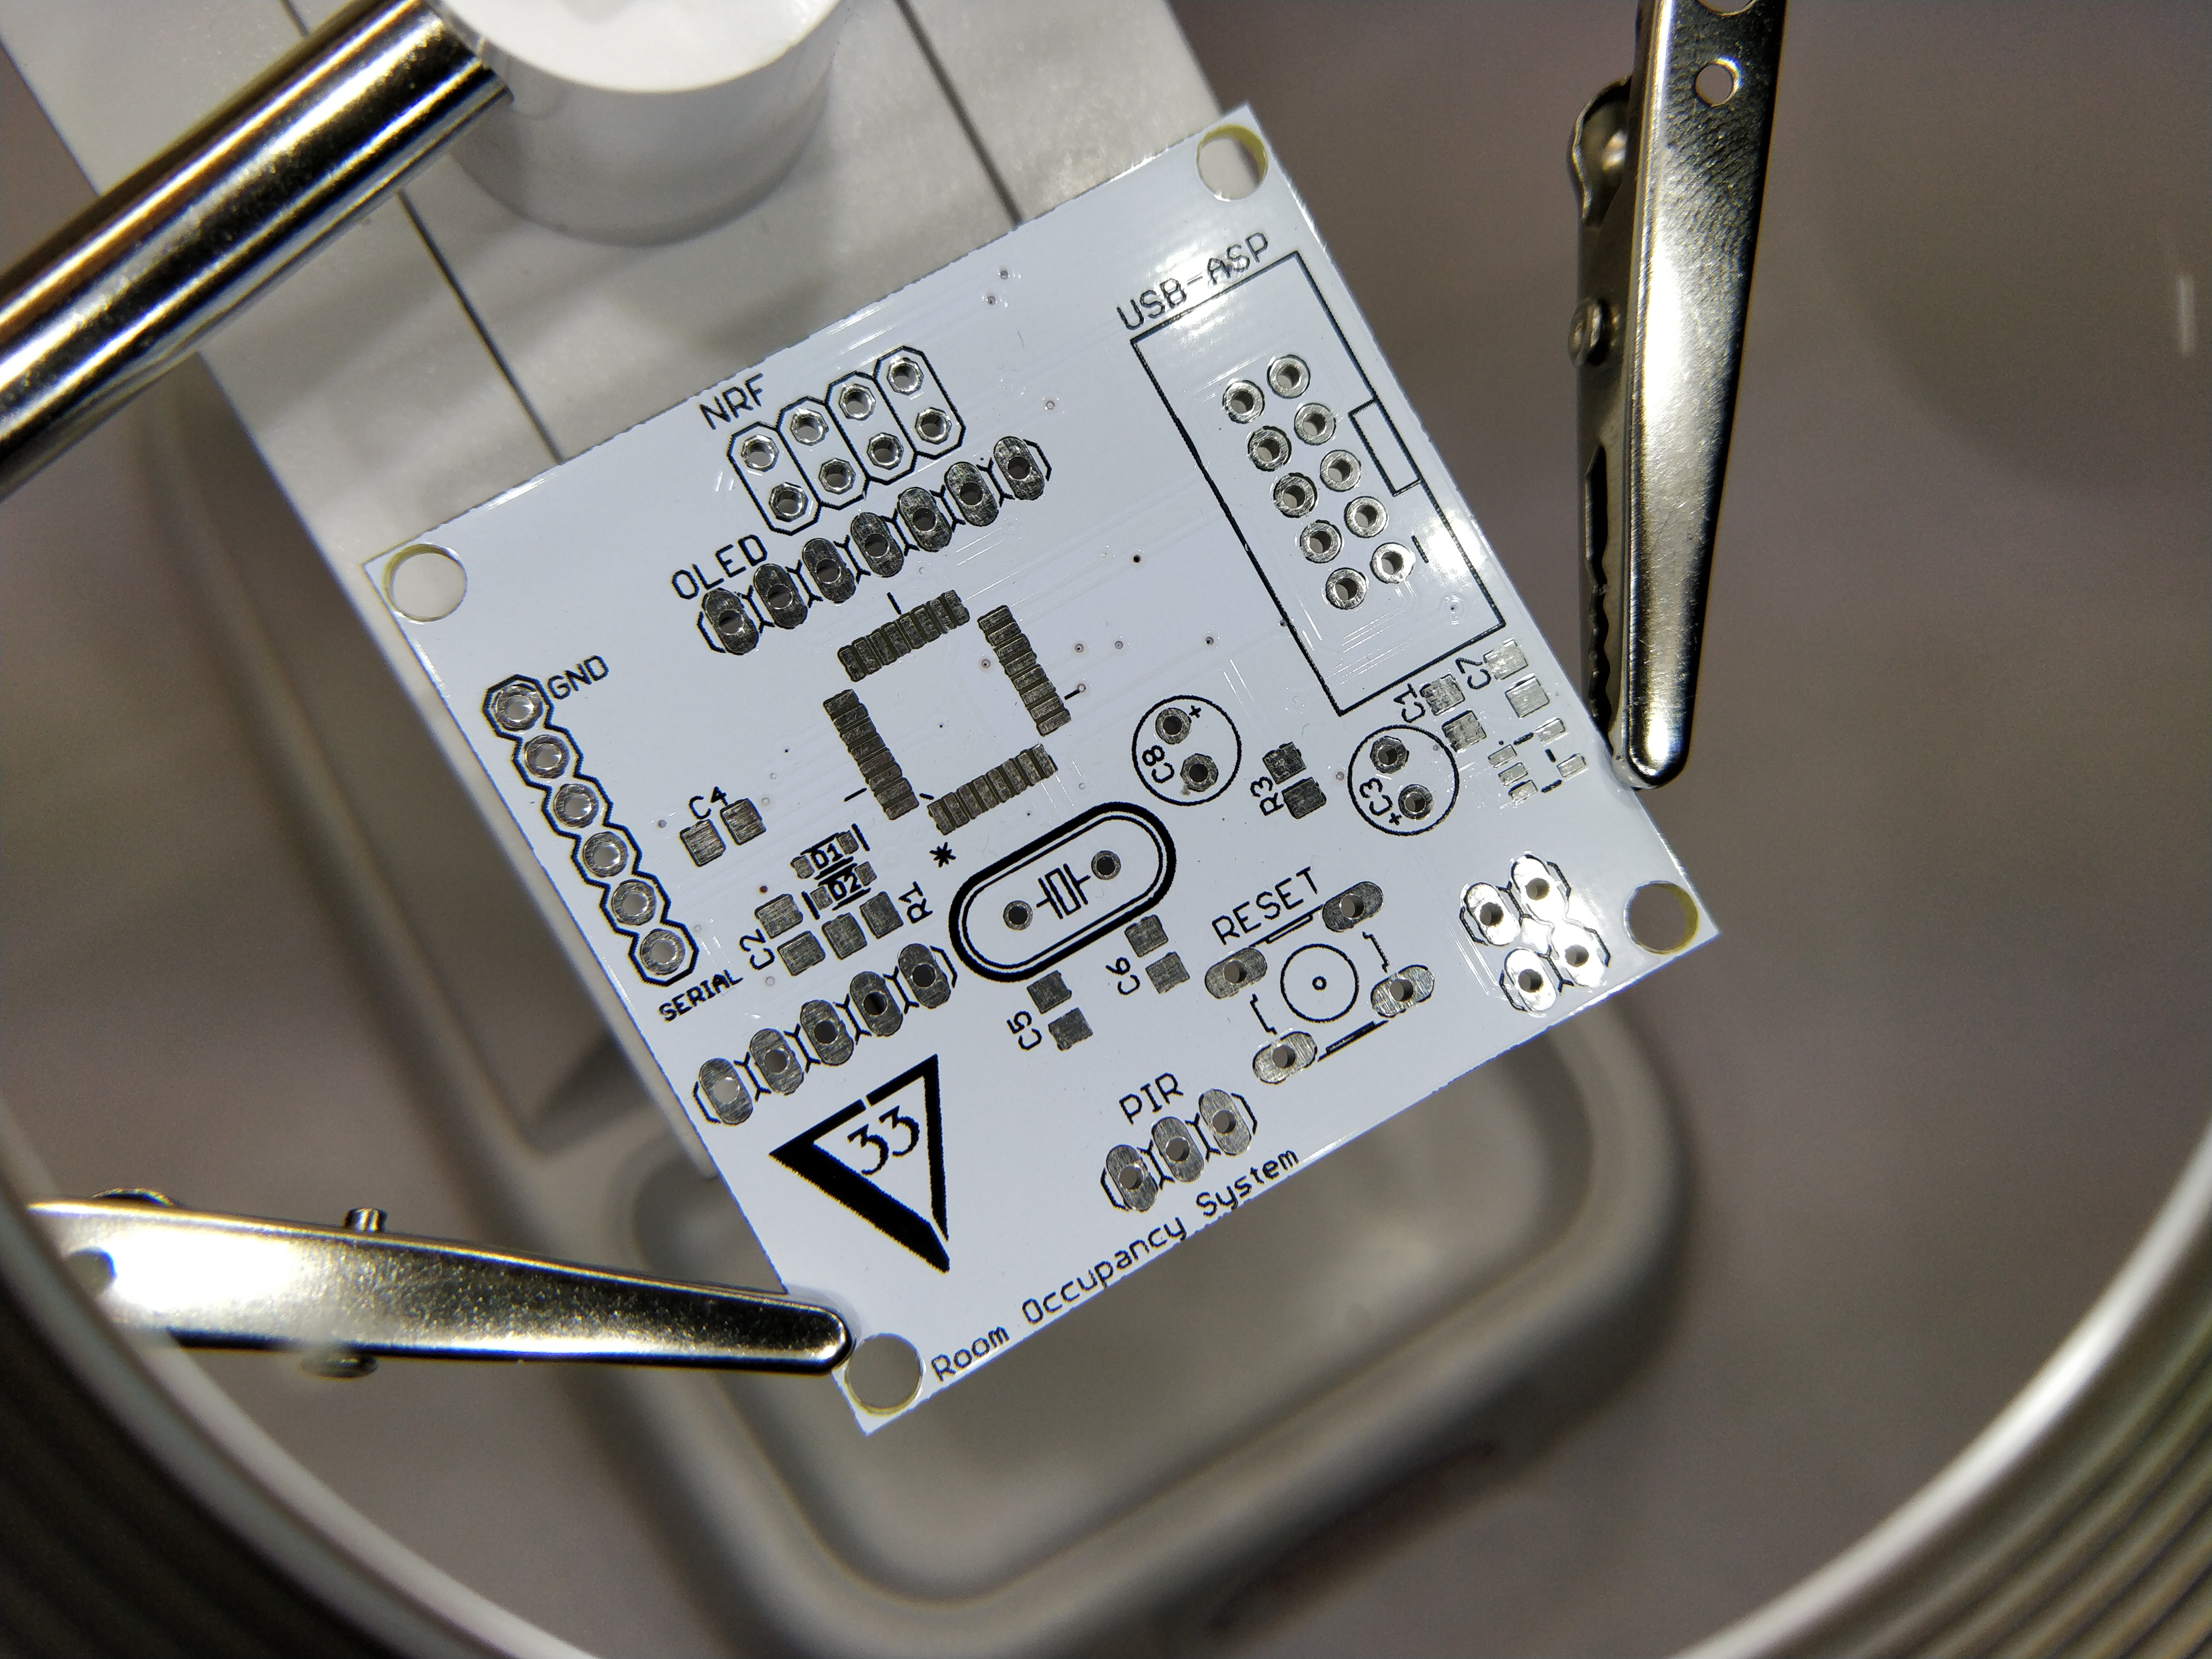
\includegraphics[scale=0.05]{PCB_3.jpg}		
		\includegraphics[scale=0.05]{PCB_2.jpg}		
		
		Populating the PCB
		
		\vspace{20pt}
		\includegraphics[scale=0.09]{AssemPCB1.jpg}
		
		Board with all the components
		
		
\end{center}

\section{3D Modelling and Print}
Any electronics project is incomplete without a proper enclosure to go with it. Normally we would have built something manually out of acrylic sheets or cardboard, but recently the institute had purchased a 3D printer, and we had multiple nodes to work with, so 3D printing an enclosure was the best option. 
We designed the 3D models by mainly taking the PCB, RF module and battery into consideration and tried to fit it a small form-factor. The modelling was done on Autodesk Fusion 360 from ground up. Pre-made models of the battery and PIR sensor was found on grabcad.com, which made the modelling process a bit easier.
After the design process, the model was exported as .stl files and sent to the printer for 3D printing. The first print of the base part failed due to a nozzle clog in the 3D printer. The second print was a success and the print turned out well, with all components falling in perfectly. Next we went ahead and printed the top half of the enclosure and it was a success as well.
The end result was a neat and aesthetically pleasing which gave the sensor nodes a product-like professional look.

\begin{center}
	\includegraphics[scale=0.25]{model.png}
	
	Designing in fusion 360	
	\vspace{15pt}
	
	\includegraphics[scale=0.25]{modelling_process.png}
	
	Modelling the enclosure as per the PCB dimensions
	\vspace{15pt}
	
	\includegraphics[scale=0.065]{3DPrint.jpg}
	\includegraphics[scale=0.05]{AssemPCB2.jpg}
	
	Printing and assembling the device
\end{center}

\section{Interface with Master Node and Web-GUI}
All packets sent from each sensor node are eventually routed to the master node, which relays it to the computer maintaining the web server. The interface between the master node and the computer is done Serially, at a baud rate of 115200 bps. The computer runs a Python script which receives all the sensor data and updates the data on the web server, which displays it to the client (browser). Timestamps are passed between the the web server and client in Unix Epoch format, while a more precise timestamp is logged locally to a text file. 
Real-time information of all the sensor nodes had to be displayed in a easy to interpret format for the user. In case of Occupeye {insert bib reference}, the sensor information is displayed on top of the map of the room itself, which makes it incredibly easy to interpret. 
{insert image of occupeye sensor state map}
Since, this is a demonstration model, and since the number of nodes is less, we do not have a fixed outline of a room available so the sensor information is just displayed on a simple browser based GUI.
The webserver was created using the Flask micro web framework, based off Python, and the client end was designed using HTML, CSS and Javascript. High speed dynamic connection between the client and server is implemented using Socket.IO. The MomentJS javascript library was used for timestamping and does the timekeeping on the client end.


\includegraphics[scale=0.25]{Website1.png}
\includegraphics[scale=0.25]{Website2.png}
\includegraphics[scale=0.25]{Website3.png}